\graphicspath{{images/stripes}}

\section{\thesection~Results}
\label{sec:results}
\citep{palkova1997}

\subsection{\thesubsection~Subsection}

\end{multicols}
\graphicspath{{images/guessing/}}
\begin{Figure}
  \centering
  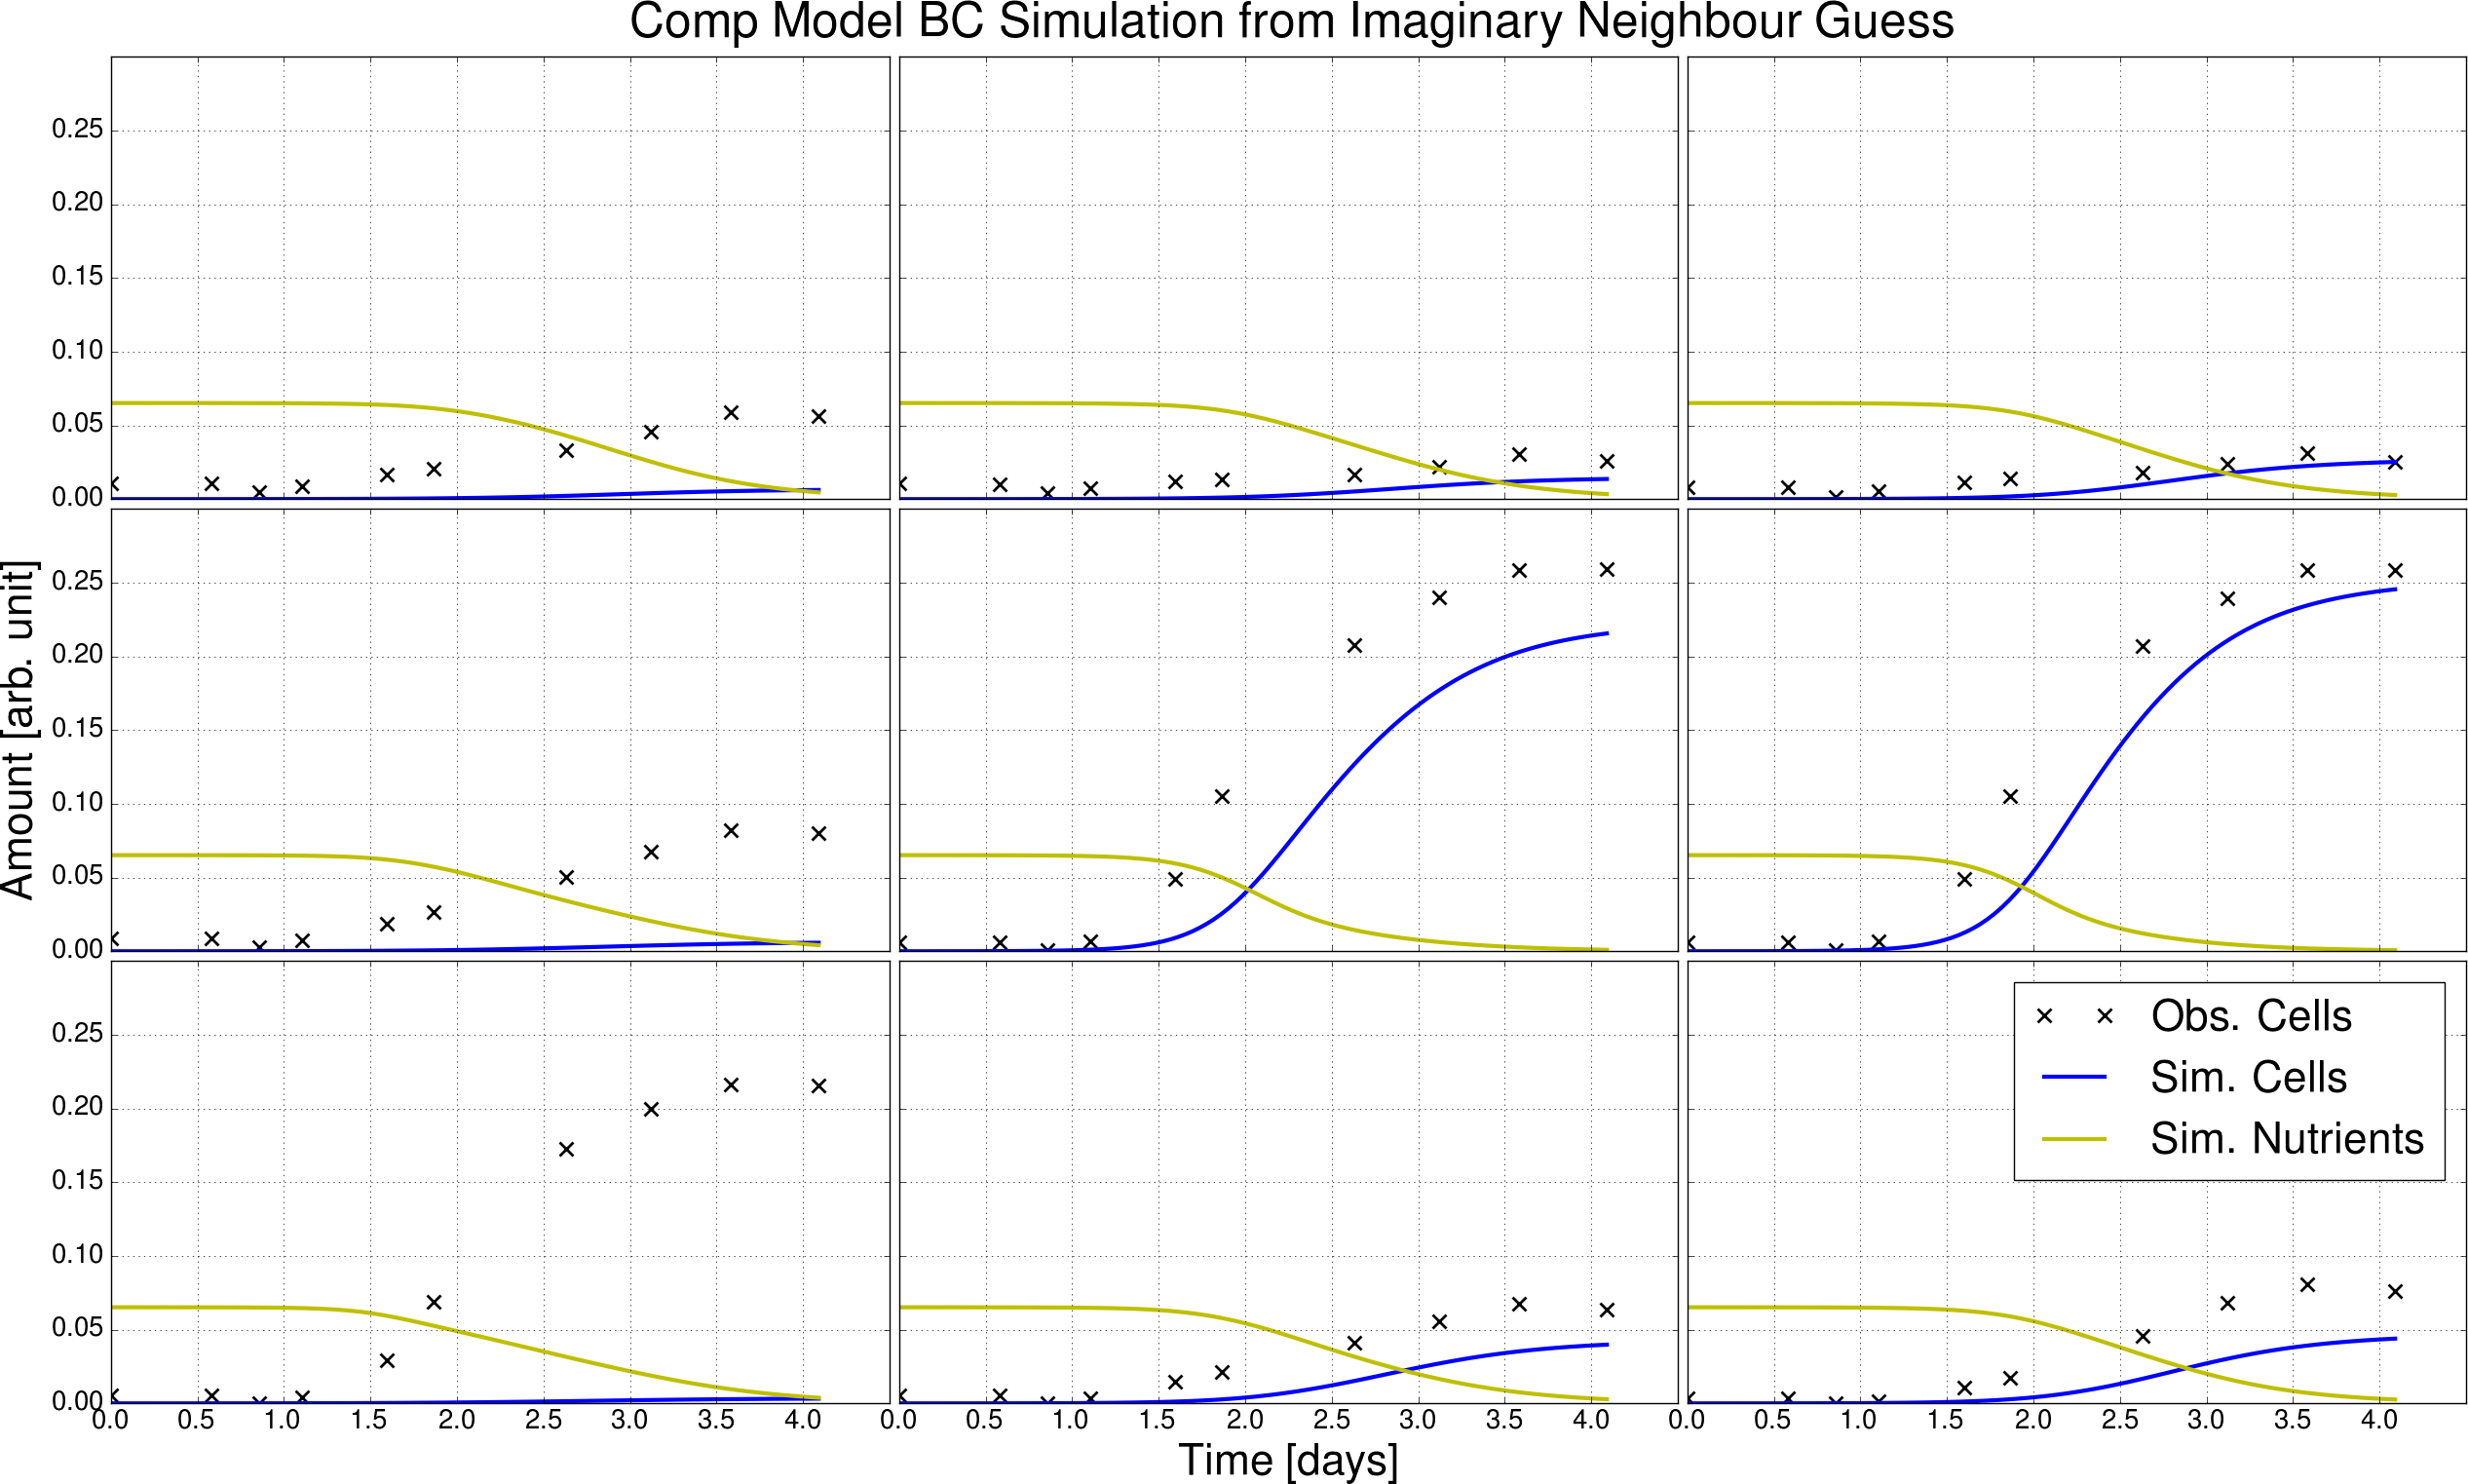
\includegraphics[width=\linewidth]{final/P15_R5_C18_guess_sim}
  \captionof{figure}{Comp Model BC simulation using parameters from
    Imaginary Neighbour guessing of P15. NOT TO GO HERE This method of
    guessing requires a b-guess to be supplied to fix the faster
    growing neighbour. (I iterated through cell ratios. I iterated
    through a range of b guesses supplied at the plate level; running
    a different script with a \(C_{0}\) guess, \(b_{guess}\). It would probably
    have been better iterate through a list of b-guess values for each
    culture and choosing the estimated b value from the best fit of
    each culture. Guessing time is currently about four minutes which
    is fast compared to fitting which takes approximately three
    hours. However, this is unlikely to stop us from encountering
    local minima when we fit the Competition Model.}
  \label{fig:imag_neigh_guess_sim}
\end{Figure}
\begin{multicols}{2}

Scripts were run with combinations of the following values.
cellratios = np.logspace(-3, -5, num=5)
fittype = ["imagneigh", "logeq"]
zerokn = [True, False]

Each script looped through the following array of b values which were
supplied to the initial guesser and used at the plate level.

for b-guess in [35, 40, 45, 50, 55, 60, 65, 70, 75, 80, 95, 100, 150]:

Each b value is used to guess a complete set of parameters b
parameters for every culture in the plate. Each of these parameter
sets is then used as an initial guess to Competition Model
fitting. For the 13 b-guesses we must run 13 Competition Model
fits. It would be better and more efficient to loop through the
b-guesses at the culture level. Each culture still undergoes imaginary
neighbour guessing with each of the 13 b-guess values, but now, for
each culture, we choose just the b estimate from the best of the 13
fits. This will produce one set of b guesses which should be superior
to any of the guesses attained when iterating through b-guess at the
plate level. Then we only need to fit the Competition Model to 1 guess
rather than 13. This will reduce the number of scripts that need to be
run in parallel, or the use of a finer grid over \(C_{0}\), and should
make convergence faster. However, if using a gradient method we are
still likely to encounter local minima from these guesses. Instead,
this improvement could be considered when developing a genetic
algorithm (if initial guesses are required) or if fitting using a
brute force method with a fine grid of fixed plate level
parameters. We will see later that with true plate level parameters
fixed we can recover good estimates for b using a gradient method. It
may be possible to evolve candidates of plate level parameters, fix
these, and minimize using the current gradient method.

% Make landscape and take a whole page.
\end{multicols}
\begin{landscape}
\graphicspath{{images/comp_fit/}}
\begin{Figure}
  \centering
  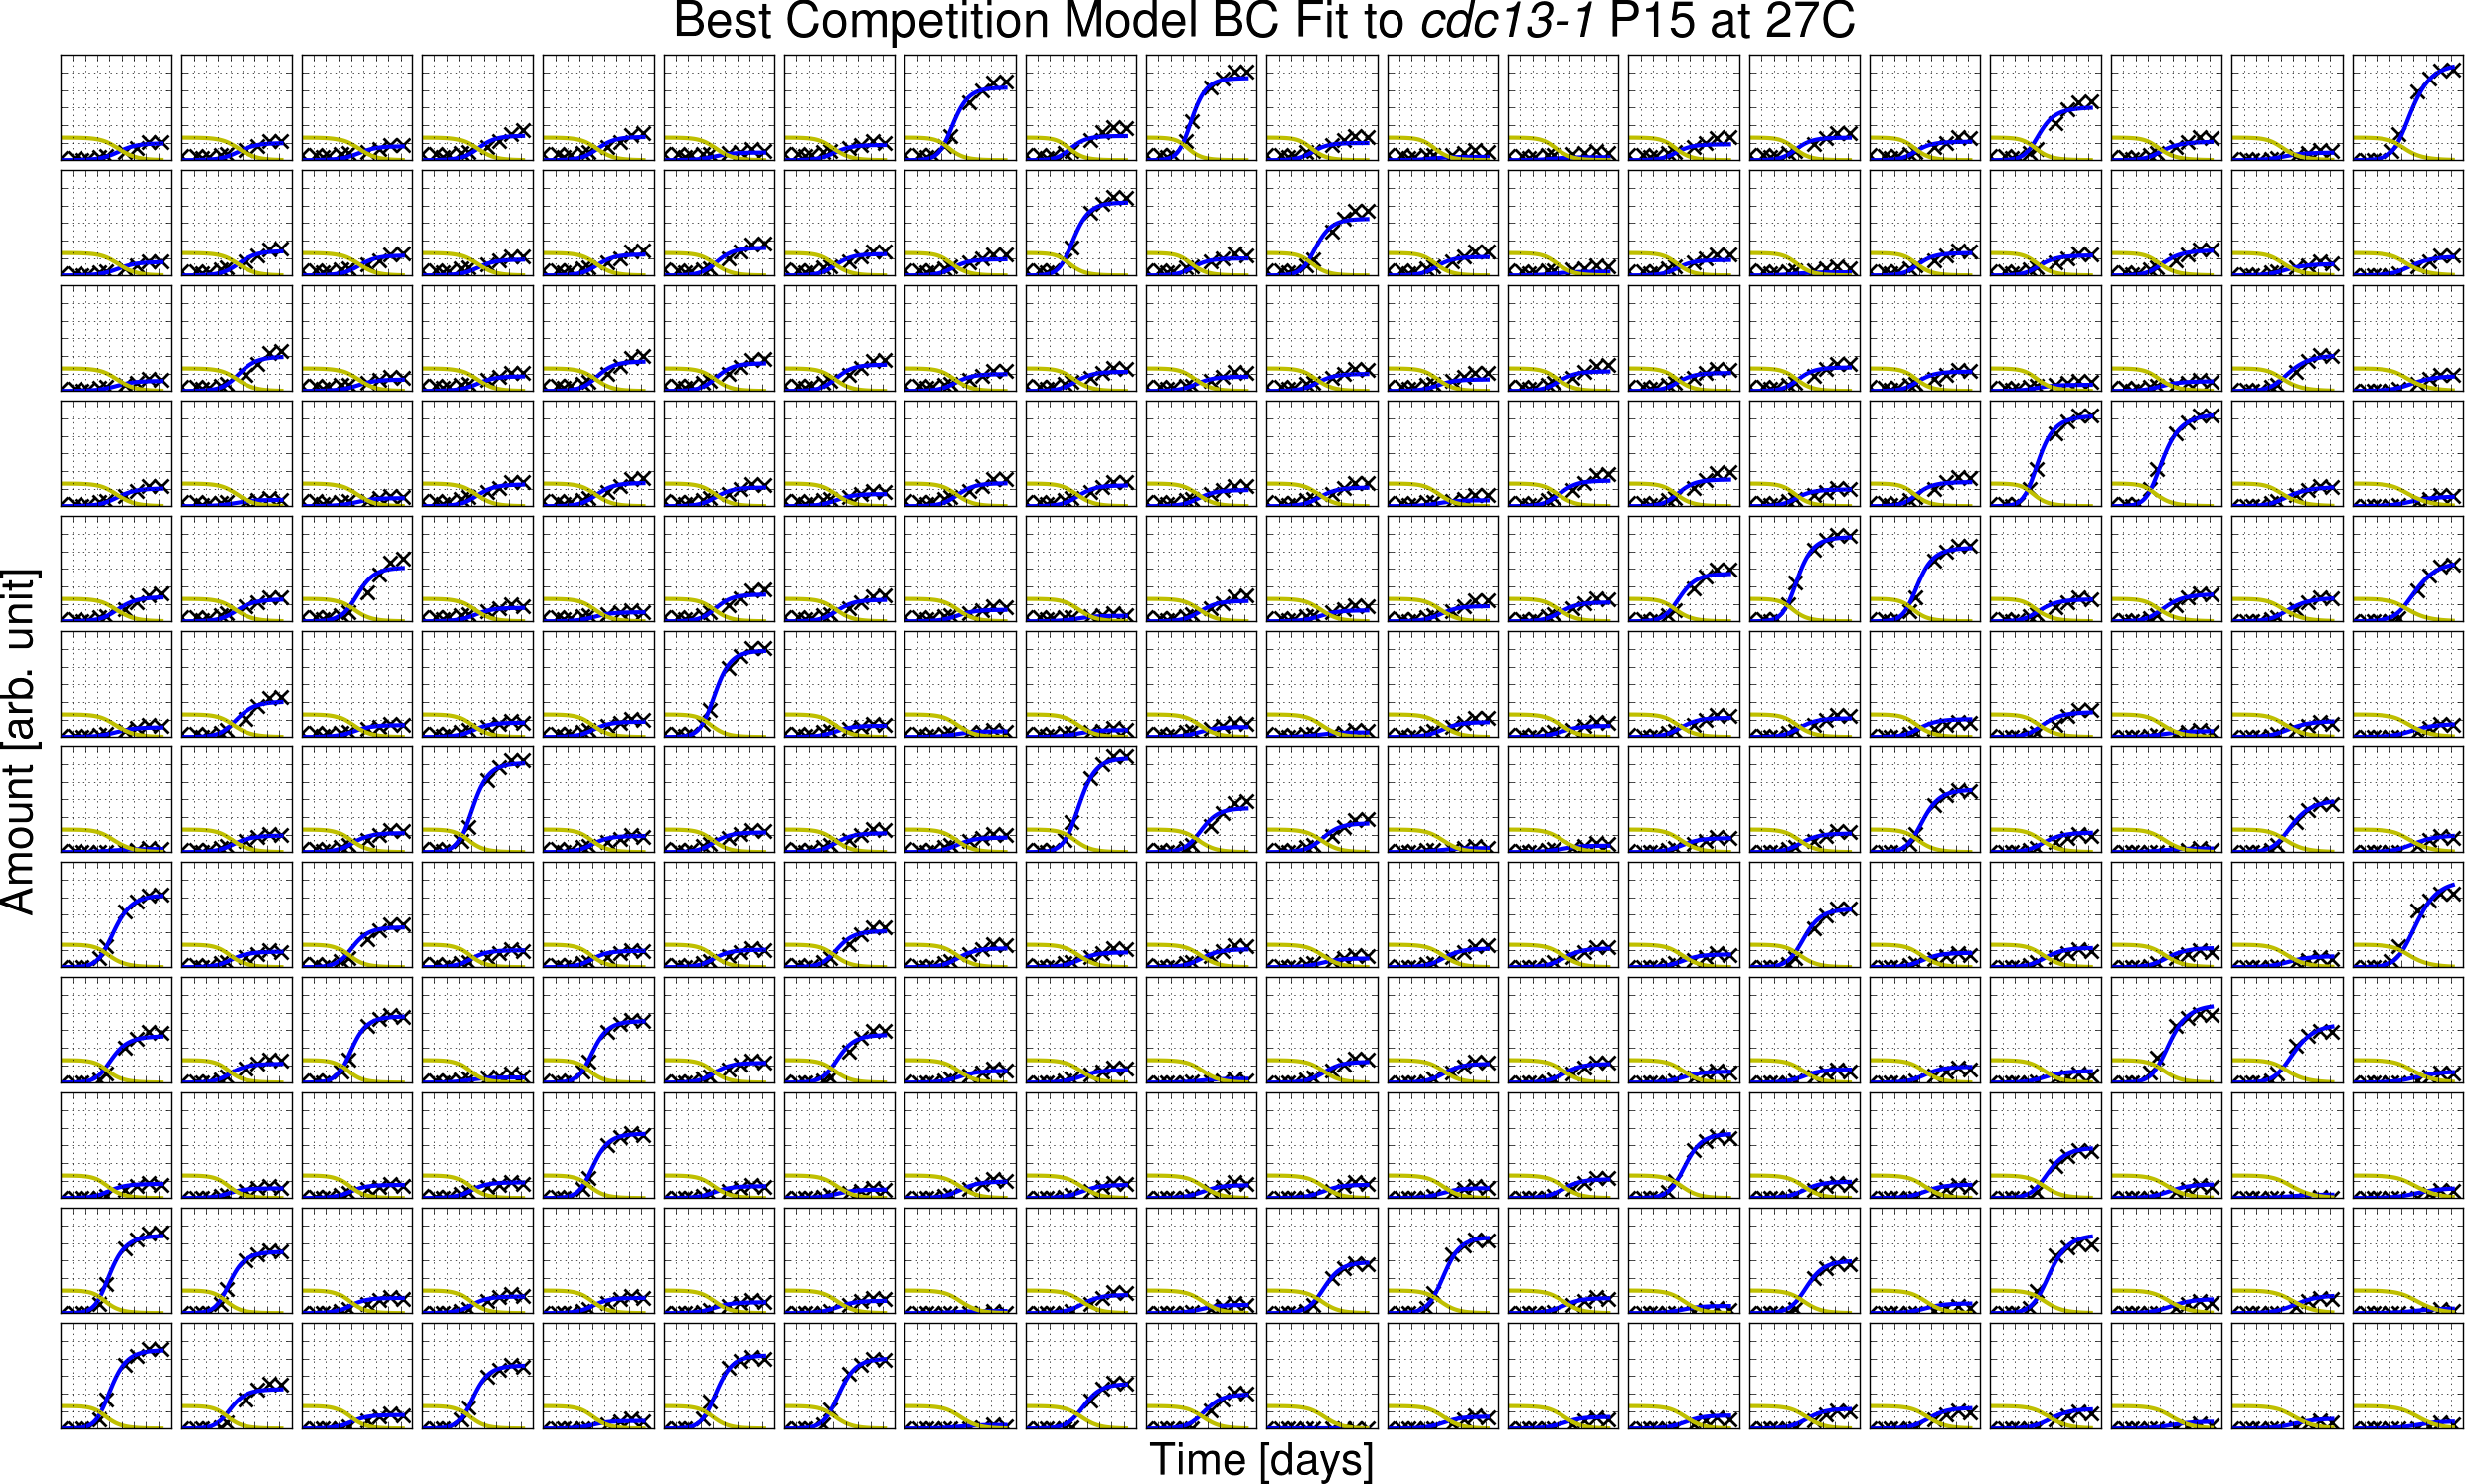
\includegraphics[width=\linewidth]{full_plate/final/P15_12x20}
  \captionof{figure}{(R5, C18) P15}
  \label{fig:comp_fit_plate}
\end{Figure}
\end{landscape}
\begin{multicols}{2}

\end{multicols}
\graphicspath{{images/comp_fit/}}
\begin{Figure}
  \centering
  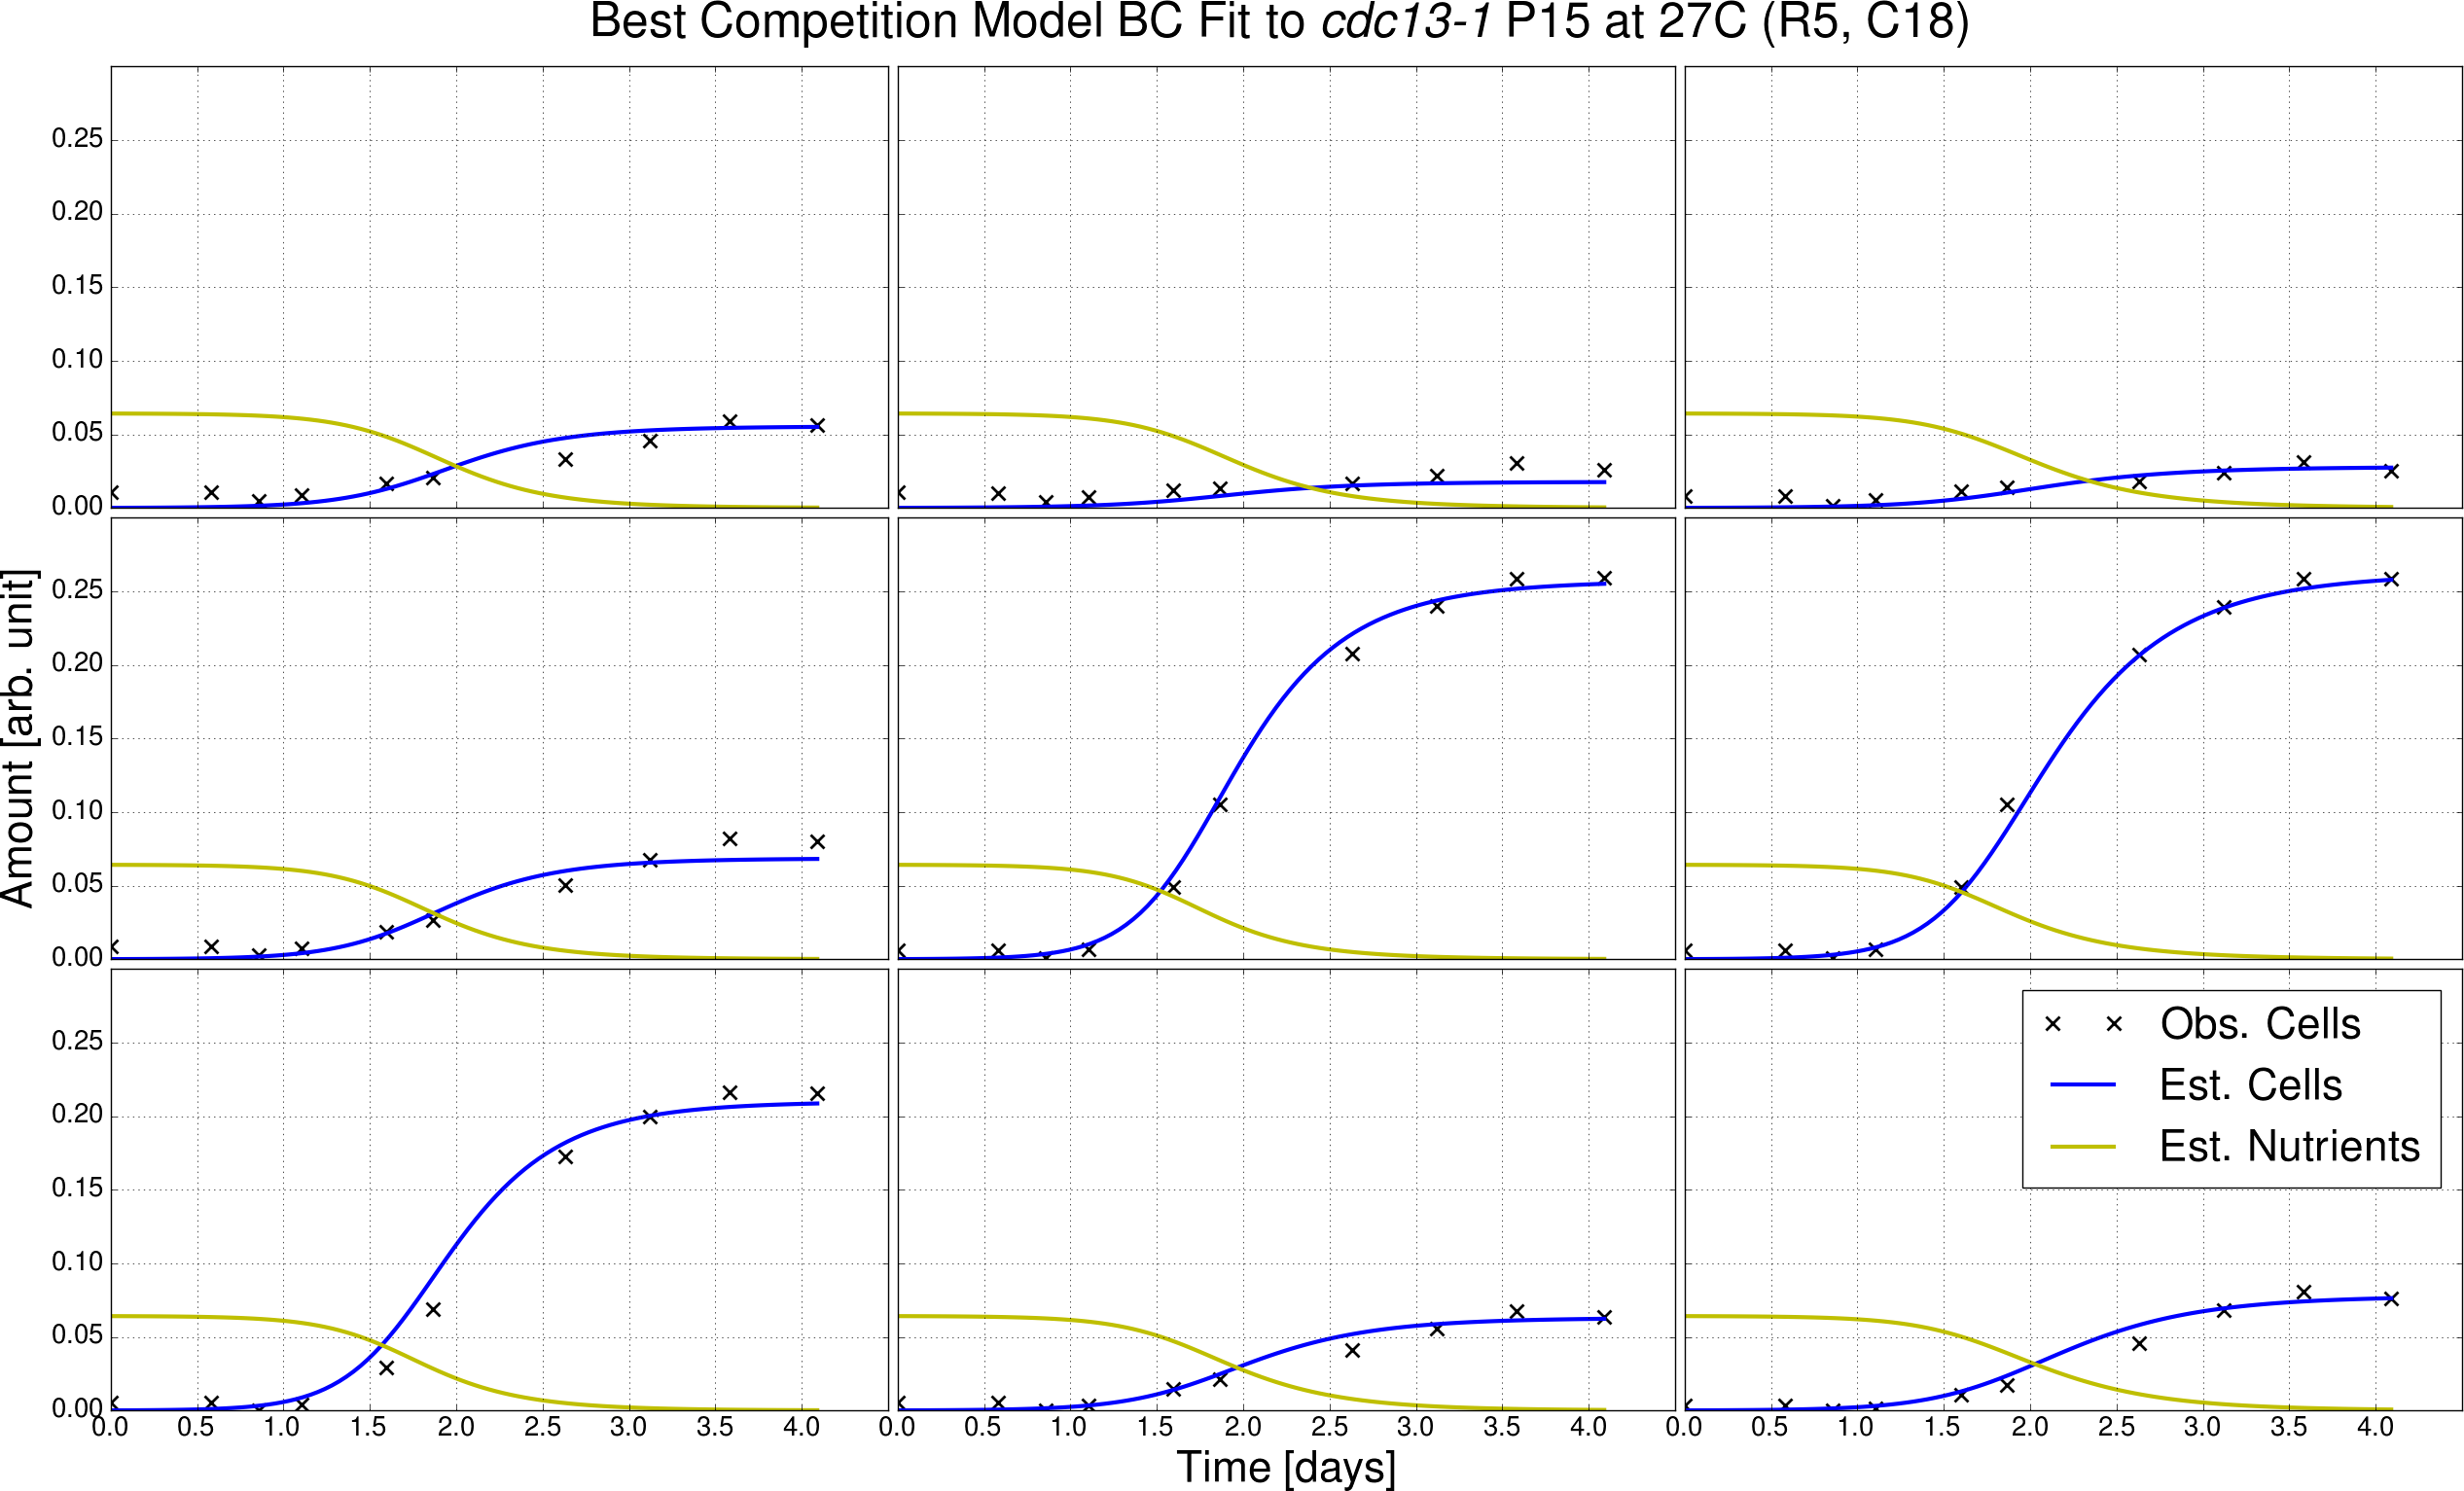
\includegraphics[width=\linewidth]{finals/P15_r5_c18_3x3}
  \captionof{figure}{(R5, C18) P15}
  \label{fig:comp_fit_zone}
\end{Figure}
\begin{multicols}{2}

\end{multicols}
\graphicspath{{images/stripes/}}
\begin{Figure}
  \centering
  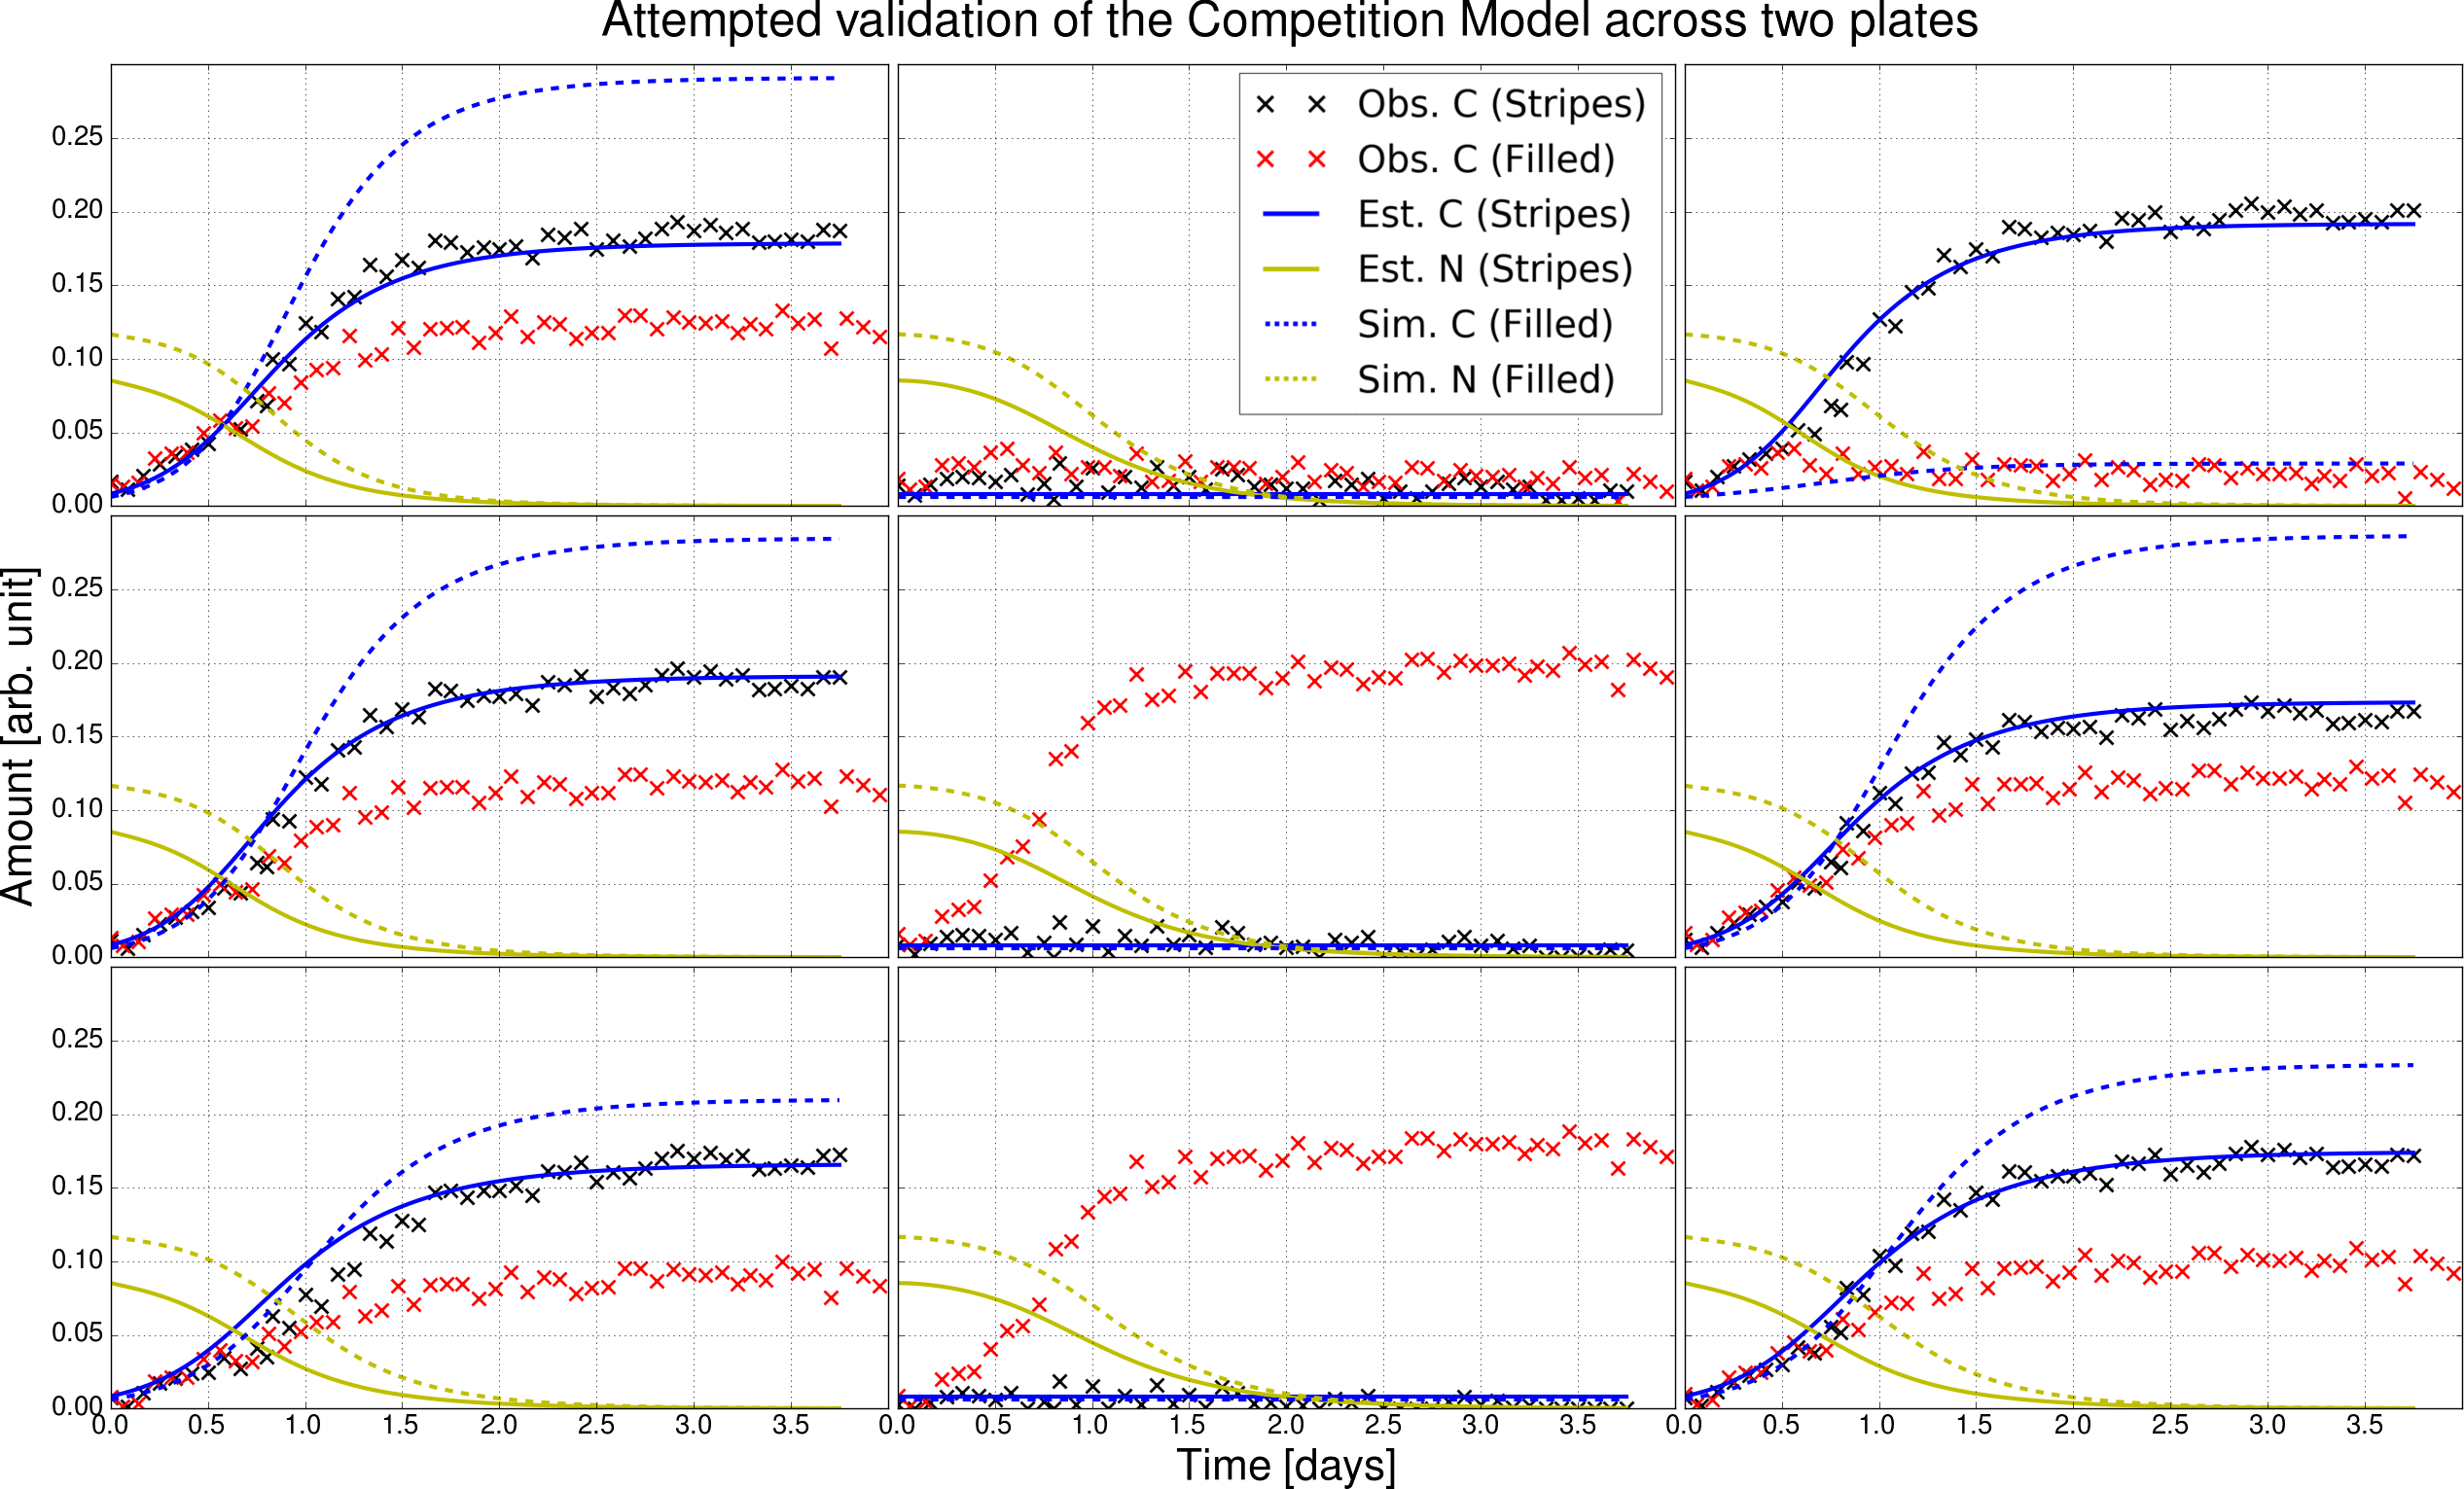
\includegraphics[width=\linewidth]{finals/validation_r9_c10}
  \captionof{figure}{(R9, C10) top-right possible pinning mistake. Bottom-left not close to any such mistake.}
  \label{fig:stripes_validation}
\end{Figure}
\begin{multicols}{2}

%%% Local Variables:
%%% mode: latex
%%% TeX-master: "report"
%%% End:
